%        File: DesignDocument.tex
%     Created: 一 3月 26 01:00 下午 2018 C
% Last Change: 一 3月 26 01:00 下午 2018 C
%
\documentclass[UTF8,noindent]{ctexart}
\usepackage[a4paper,left=2.0cm,right=2.0cm,top=2.0cm,bottom=2.0cm]{geometry}
\usepackage{hyperref}
\usepackage{url}
\usepackage{graphicx}
\usepackage{amsmath}
\usepackage{amssymb}
\usepackage{enumitem}
\usepackage{tikz}
\usepackage{float}
\usepackage{xeCJK}
\usepackage{listings}
\usepackage{xcolor}
\lstset{language = c,numbers=left, showstringspaces=false,keywordstyle= \color{ blue!70 },commentstyle=\color{red!50!green!50!blue!50}, frame=shadowbox, rulesepcolor= \color{ red!20!green!20!blue!20 } 
} 
\CTEXsetup[format={\Large\bfseries}]{section}
\usetikzlibrary{graphs}
%\newtheorem*{lemma}{Lemma}
\title{\CJKfamily{zhkai}计算机网络研讨课实验报告}
\author{{\CJKfamily{zhkai}冯吕}\ $2015K8009929049$}
\date{\today}
\begin{document}
\maketitle
\zihao{5}
\CJKfamily{zhsong}
%\begin{center}
%  \begin{tabular}{|p{15cm}|}
%    \hline
\section*{{\CJKfamily{zhhei}实验题目}}路由器转发实验
%\hline
\section*{{\CJKfamily{zhhei}实验内容}}
本次实验是静态路由器转发实验,给定网络拓扑以及节点的路由表配置,实现路由表的转发功能,使得各节点之间能够连通并传送数据。

实验内容分为两部分:
\begin{itemize}
  \item 在主机上安装arptables, iptables,用于禁止每个节点的相
	应功能,然后运行给定网络拓扑,之后,在$r1$上运行$router$,进行数据包处理,然后在$h1$上进行$ping$实验,从而判断路由器是否能够正常工作。
  \item 构造一个包含多个路由器节点组成的网络,手动配置每个路由器节点的路由表,有两个终端节点,通过路由器节点相连,两节点之间的跳数不少
	于$3$跳,手动配置其默认路由表,并通过$ping$命令和$traceroute$命令进行连通性测试和路径测试。
\end{itemize}
		%\hline
\section*{{\CJKfamily{zhhei}实验流程}}
在实验流程中,最主要的是实现路由表的转发功能。

路由器实现包含如下四个部分内容:
\begin{itemize}
  \item 处理$ARP$请求和应答;
	\item $ARP$缓存管理;
	  \item $IP$地址查找和$IP$数据包转发;
		\item 发送$ICMP$数据包
\end{itemize}
这四个部分分别有对应的一些需要实现的函数,下面我们一一来看。

\subsection*{处理$ARP$请求和应答}
路由器收到一个数据包后,如果在$ARP$缓存中找不到$IP\rightarrow MAC$映射,那么,就需要将数据包缓存到$arpcache->req\_list$中,并发送$ARP$请求。

查询函数为$arpcache\_lookup$,函数实现如下:
\begin{lstlisting}
int arpcache_lookup(u32 ip4, u8 mac[ETH_ALEN])
{
	pthread_mutex_lock(&arpcache.lock);
	for ( int i = 0; i != MAX_ARP_SIZE; ++i ){
		if (arpcache.entries[i].ip4 == ip4 
		 && arpcache.entries[i].valid){
			memcpy(mac, arpcache.entries[i].mac, ETH_ALEN);
			pthread_mutex_unlock(&arpcache.lock);
			return 1;
		}
	}
	pthread_mutex_unlock(&arpcache.lock);
	return 0;
}
\end{lstlisting}
在查找过程中,遍历$arpcache$中的所有$entry$,如果某个$entry$的$IP$和需要查询的$IP$相等并且是有效的,则把对应的$mac$复制到对应的参数中,然后返回$1$,否则返回$0$。

缓存数据包的函数为$arpcache\_append\_packet$,该函数的定义如下:
\begin{lstlisting}
void arpcache_append_packet(iface_info_t *iface, u32 ip4,
char *packet, int len)
{
	pthread_mutex_lock(&arpcache.lock);
	struct cached_pkt *new_pkt = (struct cached_pkt *)malloc(
					sizeof(struct cached_pkt));
	init_list_head(&new_pkt->list);
	if ( !new_pkt ){
		printf ("Allocate memory(new_pkt) failed.\n");
		pthread_mutex_unlock(&arpcache.lock);
		exit(0);
	}
	new_pkt->len = len;
	new_pkt->packet = packet;
	struct arp_req *pos, *q;
	list_for_each_entry_safe(pos, q, &arpcache.req_list, list){
		if(pos->iface == iface && pos->ip4 == ip4){
			list_add_tail(&new_pkt->list, &(pos->cached_packets));
			pthread_mutex_unlock(&arpcache.lock);
			return;
		}
	}
	struct arp_req *new_rep = (struct arp_req *)malloc(
					sizeof(struct arp_req));
	init_list_head(&new_rep->list);
	init_list_head(&new_rep->cached_packets);
	if (!new_rep){
		printf("Allocate memory(new_rep) falied.\n");
		pthread_mutex_unlock(&arpcache.lock);
		exit(0);
	}
	new_rep->iface = iface;
	new_rep->ip4 = ip4;
	new_rep->sent = time(NULL);
	new_rep->retries = 0;
	list_add_head(&new_pkt->list, &new_rep->cached_packets);
	list_add_tail(&(new_rep->list), &(arpcache.req_list));
	arp_send_request(iface, ip4);
	pthread_mutex_unlock(&arpcache.lock);
}
\end{lstlisting}
缓存包时,首先分配一块空间$new\_pkt$来存储包,然后,在$req\_list$中进行查找,如果其中一个$entry$的$iface$和$ip$和这一个包相同,那么说明之前就已经发送过$arp\ request$了,直接将包插入这个$entry$的尾部;否则,需要重新分配一个$entry$,然后插入,$req\_list$中,再将包插入新分配的$entry$中,这种情况下说明还没有发送过$request$,因此,之后便发送$arp\ request$。

发送$arp\ request$的函数为$arp\_send\_request$,该函数的定义如下:
\begin{lstlisting}
void arp_send_request(iface_info_t *iface, u32 dst_ip)
{
	char *packet = (char *) malloc
	(sizeof(struct ether_arp)+sizeof(struct ether_header));
	struct ether_arp *eth_arp = (struct ether_arp *)
	(packet + ETHER_HDR_SIZE);
	struct ether_header *eth_h = (struct ether_header *)(packet);
	memcpy(eth_h->ether_shost, iface->mac, ETH_ALEN);
	for (int i = 0; i != ETH_ALEN; ++i){
		eth_h->ether_dhost[i] = 0xff;
	}
	eth_arp->arp_hln = 6;
	eth_arp->arp_pln = 4;
	eth_arp->arp_hrd = htons(ARPHRD_ETHER);
	eth_arp->arp_pro = htons(ETH_P_IP);
	eth_h->ether_type = htons(ETH_P_ARP);
	eth_arp->arp_op = htons(0x0001);
	eth_arp->arp_spa = htonl(iface->ip);
	memcpy(eth_arp->arp_sha, iface->mac, ETH_ALEN);
	eth_arp->arp_tpa = htonl(dst_ip);
	iface_send_packet(iface, packet, sizeof(struct ether_arp)
	+ sizeof(struct ether_header));
}
\end{lstlisting}
在该函数中,首先,分配空间,然后构建一个$arp\ request$包,在不同字段赋上正确的值,然后使用$ iface\_send\_packet$函数将包发送出去。

处理$arp$包的函数为$handle\_arp\_packet$,该函数的定义如下:
\begin{lstlisting}
void handle_arp_packet(iface_info_t *iface, char *packet, int len)
{
	struct ether_arp *eth_arp = (struct ether_arp *)(
	packet + ETHER_HDR_SIZE);
	if (ntohs(eth_arp->arp_op) == 0x0001){
		if (ntohl(eth_arp->arp_tpa) == iface->ip){
			arpcache_insert(ntohl(eth_arp->arp_spa),
			eth_arp->arp_sha);
			arp_send_reply(iface, eth_arp);
		}
		else {
			iface_send_packet(iface, packet, len);
		}
	}
	if (ntohs(eth_arp->arp_op) == 0x0002){
		arpcache_insert(ntohl(eth_arp->arp_spa), eth_arp->arp_sha);
	}
}
\end{lstlisting}
当收到一个$arp$包时,需要根据$arp\_op$来判断收到的是$arp$请求还是$arp$应答。如果等于$1$说明是$arp$请求,则进行$reply$,否则,说明是应答,将收到的映射插入到$arpcache$中。

回复$arp$请求的函数为$arp\_send\_reply$,该函数的定义如下:
\begin{lstlisting}
void arp_send_reply(iface_info_t *iface, struct ether_arp *req_hdr)
{
	char *packet = (char *) malloc(sizeof(struct ether_arp) +
	sizeof(struct ether_header));
	struct ether_arp *eth_arp = (struct ether_arp *)(packet + 
	ETHER_HDR_SIZE);
	memcpy(eth_arp , req_hdr, sizeof(struct ether_arp));
	memcpy(eth_arp->arp_sha, iface->mac, ETH_ALEN);
	eth_arp->arp_spa = htonl(iface->ip);
	memcpy(eth_arp->arp_tha, req_hdr->arp_sha, ETH_ALEN);
	eth_arp->arp_tpa = req_hdr->arp_spa;
	eth_arp->arp_op = htons(0x0002);

	struct ether_header *eth_h = (struct ether_header *) (packet);
	eth_h->ether_type = htons(ETH_P_ARP);
	memcpy(eth_h->ether_dhost, req_hdr->arp_sha, ETH_ALEN);
	memcpy(eth_h->ether_shost, iface->mac, ETH_ALEN);
	iface_send_packet(iface, packet, sizeof(struct ether_arp) + 
	sizeof(struct ether_header));
}
\end{lstlisting}
该函数构建一个$reply$包,然后通过$iface\_send\_packet$将包发送回去。

插入新的映射的函数为$arpcache\_insert$,该函数的定义如下:
\begin{lstlisting}
void arpcache_insert(u32 ip4, u8 mac[ETH_ALEN])
{
	pthread_mutex_lock(&arpcache.lock);
	int i;
	for (i = 0; i != MAX_ARP_SIZE; ++i){
		if (arpcache.entries[i].valid == 0){
			break;
		}
		if (arpcache.entries[i].ip4 == ip4 && 
		arpcache.entries[i].valid == 1){
			arpcache.entries[i].added = time(NULL);
			pthread_mutex_unlock(&arpcache.lock);
			return ;
		}
	}
	if (i < MAX_ARP_SIZE){
		arpcache.entries[i].ip4 = ip4;
		memcpy(arpcache.entries[i].mac, mac, ETH_ALEN);
		arpcache.entries[i].added = time(NULL);
		arpcache.entries[i].valid = 1;
	}
	else {// replace the map in the first location
		arpcache.entries[0].ip4 = ip4;
		memcpy(arpcache.entries[0].mac, mac, ETH_ALEN);
		arpcache.entries[0].added = time(NULL);
		arpcache.entries[0].valid = 1;
	}
	struct arp_req *req_pos, *req_q;
	struct cached_pkt *pkt_pos, *pkt_q;
	char *packet;
	list_for_each_entry_safe(req_pos, req_q, &arpcache.req_list, list){
		if (req_pos->ip4 == ip4){
			list_for_each_entry_safe(pkt_pos, pkt_q,
			&req_pos->cached_packets, list){
				packet = pkt_pos->packet;
				struct ether_header *eth = (struct 
				ether_header *)(packet);
				memcpy(eth->ether_dhost, mac, ETH_ALEN);
				iface_send_packet(req_pos->iface, packet, 
				pkt_pos->len);
			}
			list_for_each_entry_safe(pkt_pos, pkt_q, 
			&req_pos->cached_packets, list){
				list_delete_entry(&(pkt_pos->list));
				free(pkt_pos);
			}
			list_delete_entry(&req_pos->list);
			free(req_pos);
		}//if
	}
	pthread_mutex_unlock(&arpcache.lock);
}
\end{lstlisting}
当收到新的$IP\rightarrow MAC$映射时,需要插入到$arpcache$中,首先查找是否该映射已经存在,如果已经存在,只需更新添加时间,否则,查找是否存在为$valid$的空位置,如果存在,则将映射插入该位置。如果已经满了,那么,随机选择一个映射替换出去,在这儿,我是将第一个位置的替换出去。之后,将在缓存中等待该映射的数据包,依次填写目的$MAC$地址,转发出去,并删除掉相
应缓存数据包。

\subsection*{$ARP$缓存管理}
$ARP$的管理部分,上面已经说道关于缓存查找,插入等,除此之后,还有一个就是$sweep$操作。对应的函数为$arpcache\_sweep$,该函数的定义如下:
\begin{lstlisting}
void *arpcache_sweep(void *arg) 
{
	while (1) {
		sleep(1);
		pthread_mutex_lock(&arpcache.lock);
		time_t now = time(NULL);
		for ( int i = 0; i != MAX_ARP_SIZE; ++i ){
			if ((now - arpcache.entries[i].added) > 15){
				arpcache.entries[i].valid = 0;
			}
		}
		struct arp_req *req_pos, *req_q;
		now = time(NULL);
		list_for_each_entry_safe(req_pos,
		req_q, &arpcache.req_list, list){
			if (req_pos->retries > 5){
				struct cached_pkt *pkt_pos, *pkt_q;
				list_for_each_entry(pkt_pos, 
				&req_pos->cached_packets, list){
					icmp_send_packet(pkt_pos->packet,
					pkt_pos->len, 3, 1);
				}
				list_for_each_entry_safe(pkt_pos, pkt_q,
				&req_pos->cached_packets, list){
					list_delete_entry(&pkt_pos->list);
					free(pkt_pos);
				}
				list_delete_entry(&req_pos->list);
				free(req_pos);
			}//if
			if ((now - req_pos->sent) > 1){
				arp_send_request(req_pos->iface, req_pos->ip4);
				++req_pos->retries;
			}
		}

		pthread_mutex_unlock(&arpcache.lock);
	}

	return NULL;
}
\end{lstlisting}
在该函数中,每秒中运行一次$sweep$操作,用当前时间减去缓存条目的添加时间,如果大于$15$,说明该条目在缓存中已经超过了$15$秒,则将该条目从缓存中清除,设置为无效。如果一个$IP$对应的$ARP$请求发出去已经超过了$1$秒,重新发送$ARP$请求,同时,判断发送次数是否超过了五次,如果超过五次还没有收到应答,则回复$ICMP\ Destination\ Host\ Unreachable$消息,并删除等待的数据包。同时,删除等待的数据包。

\subsection*{$IP$地址查找和$IP$数据包转发}
处理$IP$包的函数为$handle\_ip\_packet$,该函数的定义如下:
\begin{lstlisting}
void handle_ip_packet(iface_info_t *iface, char *packet, int len)
{
	struct ether_header *eh = (struct ether_header *)packet;
	struct iphdr *ip = packet_to_ip_hdr(packet);
	memcpy(eh->ether_shost, iface->mac, ETH_ALEN);
	if(ip->protocol == 1){
		struct icmphdr * icmp = (struct icmphdr *)((char *)ip +
		IP_HDR_SIZE(ip));
		if(icmp->type == 8 && iface->ip == ntohl(ip->daddr)){
			icmp_send_packet(packet, len, 8, 0);
		}
		else
		  ip_forward_packet(ntohl(ip->daddr), packet, len);
	}
	else{
		ip_forward_packet(ntohl(ip->daddr), packet, len);
	}
}
\end{lstlisting}
首先判断包是否为$ICMP$回显请求并且目的地址等于端口地址,如果是,则通过$icmp\_send\_packet$将包发送回去。否则,将该包转发出去。

进行包转发的函数为$ip\_forward\_packet$,该函数的定义如下:
\begin{lstlisting}
void ip_forward_packet(u32 ip_dst, char *packet, int len)
{
	struct iphdr *iphr = packet_to_ip_hdr(packet);
	--iphr->ttl;
	if (iphr->ttl <= 0){
		/*icmp->type = 11;*/
		/*icmp->code = 0;*/
		icmp_send_packet(packet, len, 11, 0);
		return;
	}
	rt_entry_t *dst = longest_prefix_match(ip_dst);
	iphr->checksum = ip_checksum(iphr);
	if (dst){
		/*printf(" Find ip \n");*/
		u32 next_hop = dst->gw;
		if (!next_hop){
			next_hop = ip_dst;
		}
		iface_send_packet_by_arp(dst->iface, next_hop, packet, len);
	}
	else {
		icmp_send_packet(packet, len, 3, 0);
	}
}
\end{lstlisting}
转发数据包时,首先将$TTL$值减一,如果$TTL$值变为0,则回复$ICMP$数据包。然后,重新计算校验和,通过最长前缀匹配查找转出端口,并将数据包转发出去,如果查找失败,则说明网络不可达,回复$ICMP\ Destination\ Net\ Unreachable$消息。

通过最长前缀匹配查找路由表时,将$IP$与掩码进行与运算,返回匹配长度最长的条目,如果没有匹配的条目,则说明查找失败。对应的函数为:
\begin{lstlisting}
rt_entry_t *longest_prefix_match(u32 dst)
{
	rt_entry_t *pos, *maxpos = NULL;
	u32 maxlen = 0;
	list_for_each_entry(pos,  &rtable, list){
		u32 pos_ip = pos->dest & pos->mask;
		u32 ip = dst & pos->mask;
		if ( pos_ip == ip && pos->mask > maxlen ){
			/*printf (" %d, %d\n", ip, pos_ip);*/
			maxlen = pos->mask;
			maxpos = pos;
		}
	}
	return maxpos;
	/*return NULL;*/
}
\end{lstlisting}

\subsection*{发送$ICMP$数据包}
在如下四种情况下时需要发送$ICMP$数据包:
\begin{itemize}
  \item $TTL$值减为$0$;
	\item 查找不到路由表条目,即上面说道的最长前缀匹配查找失败;
	  \item $ARP$查询失败;
		\item 收到$ping$本端口的包;
\end{itemize}
发送$ICMP$数据包的函数如下:
\begin{lstlisting}
void icmp_send_packet(const char *in_pkt, int len, u8 type, u8 code)
{
	struct ether_header *in_eth_h = (struct ether_header*)(in_pkt);
	struct iphdr *ip = packet_to_ip_hdr(in_pkt);
	int packet_len;
	char *packet;
	
	if (type == 8){
		packet_len = len;
	}
	else {
		packet_len = ETHER_HDR_SIZE+IP_BASE_HDR_SIZE+
		ICMP_HDR_SIZE+IP_HDR_SIZE(ip) + 8;
	}

	packet = (char *)malloc(packet_len);
	struct ether_header *eth_h = (struct ether_header *)(packet);
	struct iphdr *p_ip = (struct iphdr *)(packet + ETHER_HDR_SIZE);
	struct icmphdr *icmp = (struct icmphdr *)(packet + 
	ETHER_HDR_SIZE + IP_BASE_HDR_SIZE);

	memcpy(eth_h->ether_dhost, in_eth_h->ether_dhost, ETH_ALEN);
	memcpy(eth_h->ether_shost, in_eth_h->ether_dhost, ETH_ALEN);
	eth_h->ether_type = htons(ETH_P_IP);

	rt_entry_t *entry = longest_prefix_match(ntohl(ip->saddr));
	ip_init_hdr(p_ip, entry->iface->ip, ntohl(ip->saddr), 
	packet_len-ETHER_HDR_SIZE, 1);

	if (type == 8){
		char *in_pkt_rest = (char *)(in_pkt + ETHER_HDR_SIZE + 
		IP_HDR_SIZE(ip) + ICMP_HDR_SIZE - 4);
		char *packet_rest = packet + ETHER_HDR_SIZE + 
		IP_BASE_HDR_SIZE + ICMP_HDR_SIZE - 4;
		icmp->type = 0;
		icmp->code = 0;
		int data_size = len - ETHER_HDR_SIZE - IP_HDR_SIZE(ip) - 
		ICMP_HDR_SIZE + 4;
		memcpy(packet_rest, in_pkt_rest, data_size);
		icmp->checksum = icmp_checksum(icmp, data_size + 
		ICMP_HDR_SIZE - 4);
	}
	else {
		char *packet_rest = packet + ETHER_HDR_SIZE +
		IP_BASE_HDR_SIZE + ICMP_HDR_SIZE;
		icmp->type = type;
		icmp->code = code;
		int data_size = IP_HDR_SIZE(ip) + 8;
		memset(packet_rest - 4, 0, 4);
		memcpy(packet_rest, ip, data_size);
		icmp->checksum = icmp_checksum(icmp, data_size+ICMP_HDR_SIZE);
	}
	ip_send_packet(packet, packet_len);
}
\end{lstlisting}
首先,构建一个$ICMP$包,然后发送出去。在上面说到的前三种情况对应的$ICMP$数据包除了$type$和$code$不同之外,剩余部分相同。因此,在构建数据包时,需要和$ping$包进行分开讨论。如果$type$为$8$,说明收到$ping$本端口的包,此时,$ICMP$数据包的$type = 8, code = 0$,剩余部分为$ping$包中的相应字段。对于前三种情况,剩余部分则为收到数据包的头部和随后的$8$字节。\\

以上,就是路由器实现的全部内容。下面,则按照实验内容进行$ping$测试和$traceroute$测试。
\section*{{\CJKfamily{zhhei}实验结果}}
在第一部分中,$h1$能够$ping$通$h2$和$h3$,能够正确回复$ICMP$信息。
\begin{figure}[H]
  \centering
  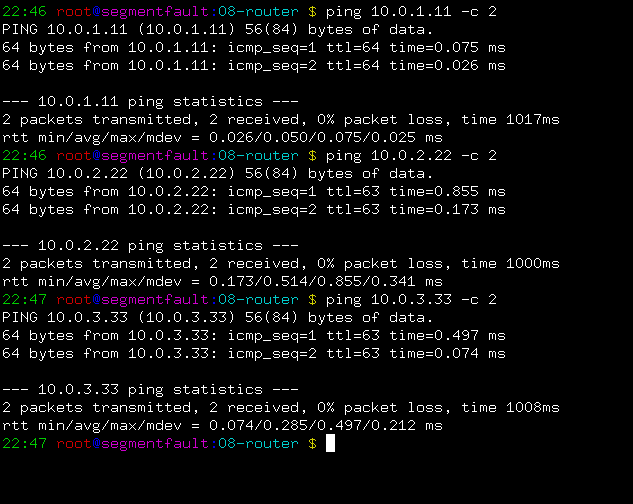
\includegraphics[scale=0.6]{1.png}
  \caption{运行截图}
\end{figure}

在第二部分,构建的网络拓扑有两个路由器节点,两个中终端节点分别连到两个路由器节点,终端节点能够$ping$通与之连接的路由器入端口,并且相互之间$traceroute$能够正确输出路径上每个节点的$IP$信息。
\begin{figure}[H]
  \centering
  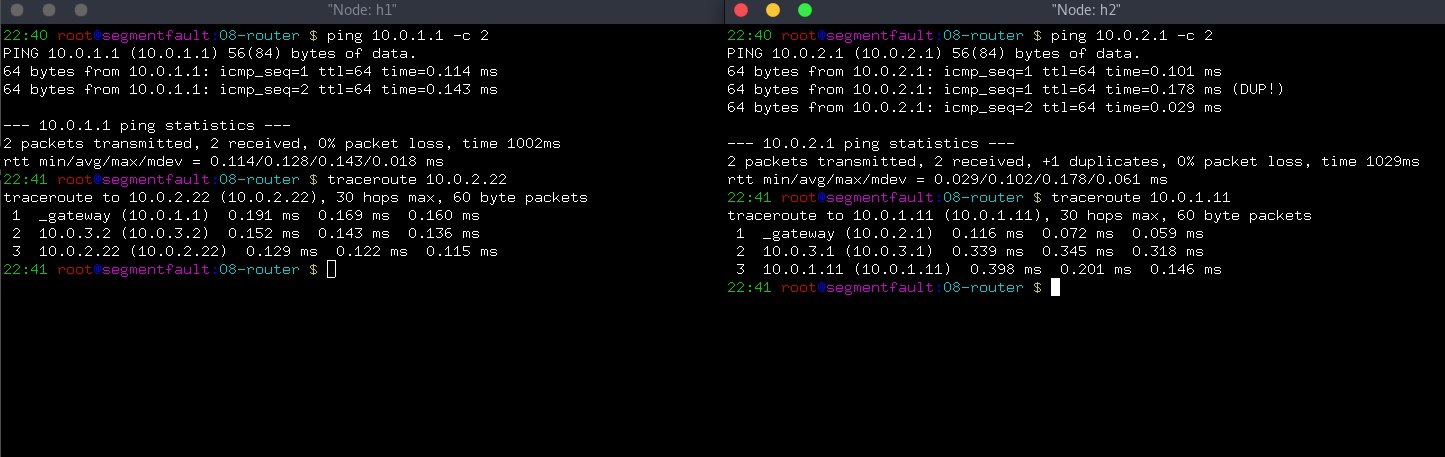
\includegraphics[scale=0.3]{2.png}
  \caption{运行截图}
\end{figure}

\section*{{\CJKfamily{zhhei}结果分析}}
在本次实验中,实验结果正确。实验需要注意的问题有,$arpcache$属于临界区的数据,因此,对它进行的操作,如插入、查找、$sweep$等都要通过锁进行互斥访问。另外,在填充包的时候,要将所有域填充完整,否则可能会倒是包的转发失败。
			%\hline
			%  \end{tabular}
			%\end{center}
\end{document}


